\documentclass[12pt]{article}
\usepackage[a4paper]{geometry}
\usepackage[myheadings]{fullpage}
\usepackage{fancyhdr}
\usepackage{lastpage}
\usepackage{graphicx, wrapfig, subcaption, setspace, booktabs}
\usepackage[T1]{fontenc}
\usepackage[font=small, labelfont=bf]{caption}
\usepackage{fourier}
\usepackage[protrusion=true, expansion=true]{microtype}
\usepackage[spanish]{babel}
\usepackage{sectsty}
\usepackage{url, lipsum}
\usepackage{graphicx}
\usepackage[utf8]{inputenc}
\usepackage{courier}
\usepackage{ulem}
\usepackage{spverbatim}
\usepackage{multirow} %para las tablas
\usepackage{color}
\usepackage{graphicx}
\usepackage{epsfig}
\usepackage{multirow}
\usepackage{colortbl}
\usepackage{xcolor}
\usepackage{float}

\usepackage{adjustbox}
\usepackage{amsmath}

\usepackage{listings} %For code in appendix
\lstset
{ %Formatting for code in appendix
    language=Matlab,
    basicstyle=\footnotesize,
    numbers=left,
    stepnumber=1,
    showstringspaces=false,
    tabsize=4,
    breaklines=true,
    breakatwhitespace=false,
}

\newcommand{\HRule}[1]{\rule{\linewidth}{#1}}
\onehalfspacing
\setcounter{tocdepth}{5}
\setcounter{secnumdepth}{5}

%-------------------------------------------------------------------------------
% HEADER & FOOTER
%-------------------------------------------------------------------------------
\pagestyle{fancy}
\fancyhf{}
\setlength\headheight{15pt}
\fancyhead[R]{PROGRAMACIÓN}
\fancyfoot[R]{\thepage}
%-------------------------------------------------------------------------------
% TITLE PAGE
%-------------------------------------------------------------------------------

\begin{document}

\title{ \normalsize \textsc{PROGRAMACIÓN}
		\\ [2.0cm]
		\HRule{2pt} \\
		\LARGE \textbf{\uppercase{Proiecto Proyectos}}
		\HRule{2pt} \\ [0.5cm] \bigskip
		\normalsize \today \vspace*{1\baselineskip}}

\date{}

\author{
        \emph{Autores:} \\ \\
		Xabier Garrote }

\maketitle
\newpage
\tableofcontents
\newpage


%--------------------------------------------------------------------% Las partes del documento de aqui en adelante ----------------------------------------------------------------------
\section{Objetivo del programa}

\section{Menu principal}
\section{Menu clientes}
\section{Menu servicios}

\newpage
\section{Manual de usuario del programa}
El programa se compone de las siguientes partes:
\subsection{El menú principal}
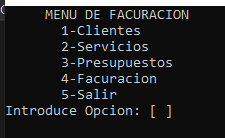
\includegraphics[]{MenuPrincipal.PNG}\\\\
En este menú el usuario tiene 4 opciones para elegir según la tarea que quiera hacer.
\begin{itemize}
    \item La 1ª opción abre el menú clientes para poder gestionar los clientes.
    \item La 2ª opción abre el menú servicios para poder gestionar los servicios.
    \item La 3ª opción abriría la pantalla de de presupuestos. Esta opción no ha podido ser implementada debido a la falta de tiempo. Es por esta razón que muestra el siguiente mensaje al pulsar en ella:\\
    
\includegraphics[]{OpcionNoImplementada.PNG} 
    \item La 4ª opción abriría la pantalla de facturación. Esta opción igual que la anterior no ha podido ser implementada debido a la falta de tiempo. Al pulsar en ella sale el siguiente mensaje:\\ 
    
\includegraphics[]{OpcionNoImplementada.PNG}
    \item La 5ª opción como su propio nombre indica es para salir del programa.
\end{itemize}

\subsection{Clientes}
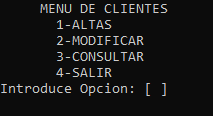
\includegraphics[]{MenuClientes.PNG}\\\\
En el menú clientes el usuario tiene tres opciones a elegir según la tarea que quiera llevar acabo.
\begin{itemize}
    \item La 1ªopcion es para dar de alta a un nuevo cliente. Al pulsar en esta opción el programa se puede encontrar con dos casos diferentes.
    \begin{itemize}
        \item El 1º caso seria que todavía no se haya ningún cliente de alta. En este caso el programa crearía un nuevo fichero llamado "\textbf{clientes.dat}". Después de crear el fichero sacaría la pantalla de petición de datos poniendo el NºCliente 1 y pidiendo al usuario que inserte el resto de datos.\\\\
        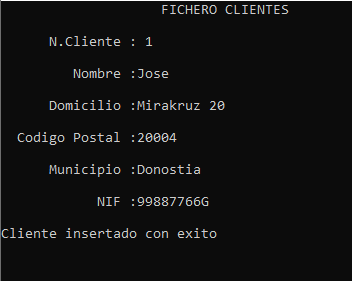
\includegraphics[]{PrimerClienteInsertado.PNG}\\\\
        Después de leer los datos insertados por el usuario el programa grabara el registro el el fichero y sacara mensaje por pantalla diciendo que el cliente se ha insertado correctamente.
        \item En el 2ºcaso seria que haya clientes dados de alta de anterioridad. En este caso el programa calculara el numero del ultimo cliente en el fichero y le sumara uno. Después sacara la pantalla de petición de datos pidiendo al usuario que inserte el resto de datos.\\\\
        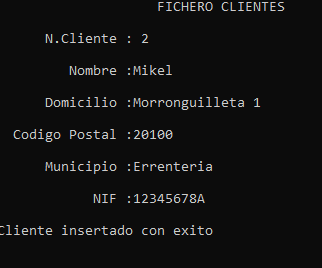
\includegraphics[]{SegundoClienteInsertado.PNG}\\\\
        Después de leer los datos insertado por el usuario el programa grabara el registro al final del fichero y sacara mensaje por pantalla diciendo que el cliente se ha insertado correctamente.
    \end{itemize}
    \item La 2ªopcion es para modificar los clientes que hay guardados. Al pulsar en esta opción el programa verifica si existe el fichero llamado "\textbf{clientes.dat}". Si no existiera daría un error indicando la no existencia del mismo. Si el fichero existe el programa pide que se introduzca un numero de cliente.\\
    
\includegraphics[]{PedirNumeroDeCliente.PNG}
    Depende el numero de cliente que se introduzca se pueden encontrar dos casos diferentes:
    \begin{itemize}
        \item 1º caso el numero de cliente introducido no existe en el fichero "\textbf{clientes.dat}". El programa mostraría el siguiente error.\\
        
\includegraphics[]{ErrorNumeroClientesNoExistente.PNG}
        \item 2º caso el numero de cliente introducido existe en el fichero.
    \end{itemize}
\end{itemize}
\end{document}